\title{Hierarchical Clustering}
\label{chp:hierarchical-clustering}
\author{Shuo Wang}
\institute{School of Computer Science, The University of Birmingham}
\maketitle

Hierarchical clustering is a type of unsupervised methods that partitions data examples into clusters without asking for the number of clusters before training starts. Unlike K-means, hierarchical clustering instead requires specifying a dissimilarity measure between groups of examples, and produces a hierarchical representation (a dendrogram) of examples showing which two groups of examples are closer at each level of the hierarchy. Strategies for hierarchical clustering divide into two types: \textit{agglomerative} (bottom-up) and \textit{divisive} (top-down). Agglomerative clustering starts at the bottom treating each single example as a cluster, and recursively merges the closest pair of clusters into a single cluster. Divisive clustering acts in the opposite direction. It starts at the top with one big cluster and recursively splits into two new groups with the largest between-group dissimilarity. Divisive clustering is less popular than agglomerative clustering due to its complexity of looking for the best split at each round, but it can be made faster. Most agglomerative clustering methods have time complexity $\mathcal{O}(N^3)$, while the fastest divisive clustering takes only $\mathcal{O}(N)$ time. In addition, divisive clustering makes splitting decisions in view of all the data examples, while the agglomerative clustering makes myopic merge decisions~\cite{Murphy2012}. 

\section{Agglomerative Clustering}
\label{sec:agglo-cluster}


Agglomerative clustering begins with every data example representing a singleton cluster. For a dataset with $N$ examples, the closest two clusters are merged into one cluster at each step, which repeats $N-1$ steps in total. When the training process ends, there is one single cluster containing all the examples. To decide the closeness of two clusters, two parameters are required: 1) a distance measure indicating how far one example is from another in a dataset; 2) a dissimilarity measure indicating the distance between two clusters. The calculation of the dissimilarity measure for clusters needs the distance measure for examples. More details about these two parameters are given in Section~\ref{subsec:dissimilarity}. The pseudocode of agglomerative clustering is given below:


%%%%%%%%%%%%%%%%%%%%%%%% ALGORITHM
\begin{algorithm}[ht!]
	%\renewcommand{\baselinestretch}{0.8}
	\caption{Agglomerative clustering}
    
    Parameters: dissimilarity measure $d$ for clusters and distance measure $d'$ for examples
    
    Output: a hierarchical data representation.
    
	\begin{algorithmic}[1] 
		\STATE{Initialize $N$ clusters $C_1, C_2, \dots, C_i, \dots, C_N$, where each cluster contains only one example.} 
		
        \REPEAT
		
		%\FOR{each model $m$}
		
		\STATE Find two closest clusters $C_j$ and $C_k$ with smallest $d$ to merge based on $d'$.
		\STATE Create a new cluster $C_l \leftarrow C_j \cup C_k$.
		\STATE Remove $C_j$ and $C_k$ from the cluster set. 
		\STATE Add $C_l$ into the cluster set. 
				
		%\ENDFOR
		\UNTIL no more clusters are available for merging.
		
	\end{algorithmic}
	
\end{algorithm}
%%%%%%%%%%%%%%%%%%%%%%%% ALGORITHM

\subsection{Dissimilarity Measures Between Clusters}
\label{subsec:dissimilarity}

To find the closest (i.e. least dissimilar) clusters at each step, a dissimilarity measure between two clusters must be defined. Different measures can give quite different results. The 3 most commonly used measures are single linkage (SL), complete linkage (CL) and group average (GA). Others exist, such as the centroid method and the Ward's method~\cite{Ward1963}. 

For any pair of clusters $C_j$ and $C_k$, the \textit{single linkage} measure $d_{SL}$, also called nearest neighbour, is defined as the distance between the two closest examples of each cluster (see Fig.~\ref{fig:sl}):
\[
d_{SL}\left ( C_j, C_k \right ) = \min_{\mathbf{x}^{\left ( t \right )} \in C_j, \mathbf{x}^{\left ( t' \right )} \in C_k} \left\{ d_{t,t'} \right\}
\]

\noindent
where $d_{t,t'}$ can be any distance measure between two examples $\mathbf{x}^{\left ( t \right )}$ and $\mathbf{x}^{\left ( t' \right )}$, such as Euclidean, Manhattan and Minkowski distances. Euclidean distance is the most commonly used one. It is defined as the length of the line between two points, and can be calculated using the Pythagorean theorem from the Cartesian coordinates of the points. The single linkage measure simply chooses the nearest examples and does not take in any account the internal cohesion of the clusters. If a small cluster is initially formed, it can lead to the progressive merging of adding one example at a time to this cluster, which is called a chain effect~\cite{Marini2020}. In fact, two clusters to be merged based on single linkage do not have to be ``compact". Compactness here means that all the examples within a group are similar to each other.

\begin{figure}[htp]
\centering
\captionsetup{justification=centering}
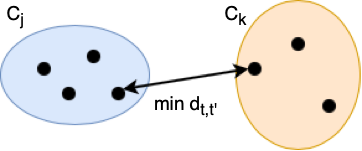
\includegraphics[width=6cm]{"Part 3 - Learning Systems/Unsupervised Learning/Hierarchical Clustering/figures/SingleLinkage.png"}
\caption{Single linkage}
\label{fig:sl}
\end{figure}

The \textit{complete linkage} measure $d_{CL}$, also called furthest neighbour technique, is defined as the distance between the two most distant examples of each cluster (see Fig.~\ref{fig:cl}):
\[
d_{CL}\left ( C_j, C_k \right ) = \max_{\mathbf{x}^{\left ( t \right )} \in C_j, \mathbf{x}^{\left ( t' \right )} \in C_k} \left\{ d_{t,t'} \right\}
\]

\begin{figure}[htp]
\centering
\captionsetup{justification=centering}
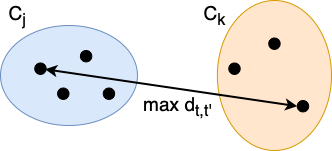
\includegraphics[width=6cm]{"Part 3 - Learning Systems/Unsupervised Learning/Hierarchical Clustering/figures/CompleteLinkage.png"}
\caption{Complete linkage}
\label{fig:cl}
\end{figure}

Complete linkage works the opposite to single linkage. Two clusters with the smallest ``furthest example distance" will be merged together at each iteration. It means that the examples from these two clusters are more compact and relatively similar. 

The \textit{group average} measure (or average linkage), uses the average distance between all pairs of examples from the two clusters (see Fig.~\ref{fig:ga}): 
\[
d_{GA}\left ( C_j, C_k \right ) = \frac{1}{N_j N_k}\sum_{\mathbf{x}^{\left( t \right )} \in C_j}\sum_{\mathbf{x}^{\left( t' \right )} \in C_k} \left\{ d_{t,t'} \right\}
\]

\noindent
where $N_j$ and $N_k$ are the number of examples in clusters $C_j$ and $C_k$ respectively. The group average is a measure in between single and complete linkage. It tends to produce more compact clusters than single linkage and further apart clusters than complete linkage.

\begin{figure}[htp]
\centering
\captionsetup{justification=centering}
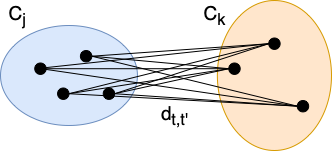
\includegraphics[width=6cm]{"Part 3 - Learning Systems/Unsupervised Learning/Hierarchical Clustering/figures/GroupAverage.png"}
\caption{Group average}
\label{fig:ga}
\end{figure}

\section{Divisive Clustering}
\label{sec:div-cluster}

Divisive clustering begins with the whole dataset as a single cluster, and then recursively splits each existing cluster into two children clusters, which have the largest between-group dissimilarity, in a top-down fashion. The pseudocode of divisive clustering is given below for a dataset with $N$ examples:

%%%%%%%%%%%%%%%%%%%%%%%% ALGORITHM
\begin{algorithm}[ht!]
	%\renewcommand{\baselinestretch}{0.8}
	\caption{Divisive clustering}
    
    Parameters: cluster choosing scheme $m$, cluster splitting scheme $s$
    
    Output: a hierarchical data representation.
    
	\begin{algorithmic}[1] 
		\STATE{All the examples $\mathbf{x}^{\left ( i \right )}$ ($i = 1, 2, \ldots, N$) form one cluster.} 
		
        \REPEAT
		
		%\FOR{each model $m$}
		
		\STATE Pick one existing cluster $C_i$ according to $m$.
		\STATE Find two furthest sub-clusters $C_j$ and $C_k$ according to $s$.  
		\STATE Create two new clusters $C_j$ and $C_k$, where $C_j \cup C_k = C_i$. 
		\STATE Remove $C_i$ from the cluster set. 
		\STATE Add $C_j$ and $C_k$ into the cluster set. 
				
		%\ENDFOR
		\UNTIL the desired number of clusters is obtained.
		
	\end{algorithmic}
	
\end{algorithm}
%%%%%%%%%%%%%%%%%%%%%%%% ALGORITHM

There are various ways to choose which cluster to be split at step 3, such as the cluster with most examples or the one with the least overall similarity among its examples. The existing research has shown that the differences between the choosing schemes were very small~\cite{Steinbach2000}. 

The splitting scheme can be any of the combinatorial methods, such as K-means with $K=2$. This clustering procedure combining divisive clustering and K-means is called the bisecting K-means algorithm~\cite{Steinbach2000}. However, such schemes would depend on the algorithm initialization specified at each step. In addition, they do not necessarily hold the monotonicity property required for dendrogram representation~\cite{Hastie2009}. A method called \textit{dissimilarity analysis} proposed by Macnaughton-Smith et al. avoids these problems~\cite{Macnaughton-Smith1964}. Instead of considering all divisions, it starts with a single cluster $C_j$ containing all the data examples, then measures the average dissimilarity of each example $\mathbf{x}^{\left( t \right )}$ to all the other examples in $C_j$. The example that has the largest average dissimilarity is then moved to a second cluster $C_k$. The above is repeated, i.e. moving examples from $C_j$ to $C_k$, until the example in $C_j$ with the largest average dissimilarity to the examples in $C_j$ has a smaller average dissimilarity than its average dissimilarity to the examples in $C_k$. That is, there is no more examples in $C_j$ that are on average closer to $C_k$. This process results in two children clusters. Each successive hierarchical level is produced by applying this process to each of the clusters at the previous level. Based on the dissimilarity analysis method, Kaufman and Rousseeuw proposed DIANA (Divisive ANAlysis). It splits a cluster by moving examples from a larger sub-cluster to a smaller one. The move occurs when the average dissimilarity of an example $\mathbf{x}^{\left( t \right )}$ in the larger sub-cluster to the remaining examples in that sub-cluster is larger than the average dissimilarity of $\mathbf{x}^{\left( t \right )}$ to the examples in the smaller sub-cluster~\cite{Kaufman1990}. A comparison between agglomerative and divisive clustering can be found here~\cite{Kumar2020}. 


\section{Interpreting a Dendrogram}
\label{sec:dendro}

The binary tree produced by hierarchical clustering is called a dendrogram. It is a graphical display of how examples are grouped at each hierarchy level. A dendrogram is highly interpretable, which is one of the main reasons for the popularity of hierarchical clustering. 

Let's begin with a simple example. It is a simulated data set with 5 two-dimensional examples, as shown in Fig.~\ref{fig:data}. 

\begin{figure}[htp]
\centering
\captionsetup{justification=centering}
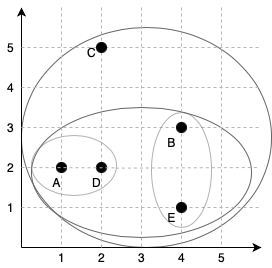
\includegraphics[width=6cm]{"Part 3 - Learning Systems/Unsupervised Learning/Hierarchical Clustering/figures/Dendrogram-Data.png"}
\caption{Two-dimensional data examples}
\label{fig:data}
\end{figure}

If we apply agglomerative clustering with single linkage, the clustering happens in the following order:
\begin{enumerate}
\item Examples A and D are grouped with distance 1. 
\item Examples B and E are grouped with distance 2. 
\item Cluster (A, D) and Cluster (B, E) are grouped with distance $\sqrt{5}$. 
\item Example C is merged to Cluster (A, D, B, E) with $2\sqrt{2}$. 
\end{enumerate}

The resulting dendrogram is shown in Fig.~\ref{fig:dendro}. The horizontal axis indicates the examples in the dataset. The links between the examples represent which examples are merged into one cluster. The vertical axis represents the height of two merging clusters. \textit{Height} is referred to as the distance/dissimilarity between the clusters. In this case, the distance between A and D is 1; thus, their connecting line is at 1 along the vertical axis. Similarly, B and E are connected at the height of 2. This height is monotonically increasing with the level of the dendrogram. In other words, the examples that merge at the very bottom of the tree are quite similar, whereas the examples that merge close to the top of the tree tend to be very different. 

\begin{figure}[htp]
\centering
\captionsetup{justification=centering}
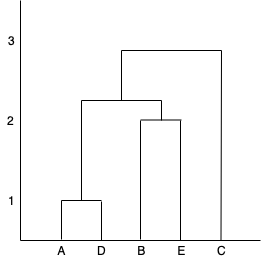
\includegraphics[width=6cm]{"Part 3 - Learning Systems/Unsupervised Learning/Hierarchical Clustering/figures/Dendrogram.png"}
\caption{Resulting dendrogram}
\label{fig:dendro}
\end{figure}

Dendrograms should be read with caution. First, different hierarchical methods and dissimilarity measures can lead to quite different dendrograms. Second, when reading a dendrogram, we cannot conclude about the similarity of two examples based on how far they are along the horizontal axis~\cite{James2013}. For example, example C in Fig.~\ref{fig:dendro} locates next to example E, but it does not mean C closer to E. All the other examples are in fact closer to C. Third, hierarchical clustering does not tell you the ``right" number of clusters. Instead, it creates a hierarchical representation of data, even if data has absolutely no hierarchical meanings. By cutting off a dendrogram at various heights, different numbers of clusters are obtained. In practice, people often look at the dendrogram and select by eye a sensible number of clusters, based on the heights of merging clusters and the desired number of clusters~\cite{James2013}. Alternatively, other approaches have to be used, such as Bayesian hierarchical clustering~\cite{Heller2005}.

\section{Example: Yeast Gene Data}

Agglomerative clustering is popular in bioinformatics, because it provides visualization of clusters as dendrogram and gives explainability to the task. Here, we use a yeast gene expression dataset~\cite{Kaggle2016} and aim to cluster similar yeast samples together. It contains 92 samples described by over 6000 genes. 

Fig.~\ref{fig:example} shows the dendrograms resulting from agglomerative clustering with single linkage, complete linkage and group average respectively. Depending on which dissimilarity measure we use, the results are quite different. The generated binary trees are more balanced in the complete linkage and group average cases than in the single linkage case. In practice, the choice of dissimilarity measure should take into consideration the type of data and the learning task at hand~\cite{James2013}. The vertical axis in each dendrogram shows the height of two clusters when they are merged. 

\begin{figure}[htp]
  \centering
  \begin{subfigure}[b]{0.8\linewidth}
    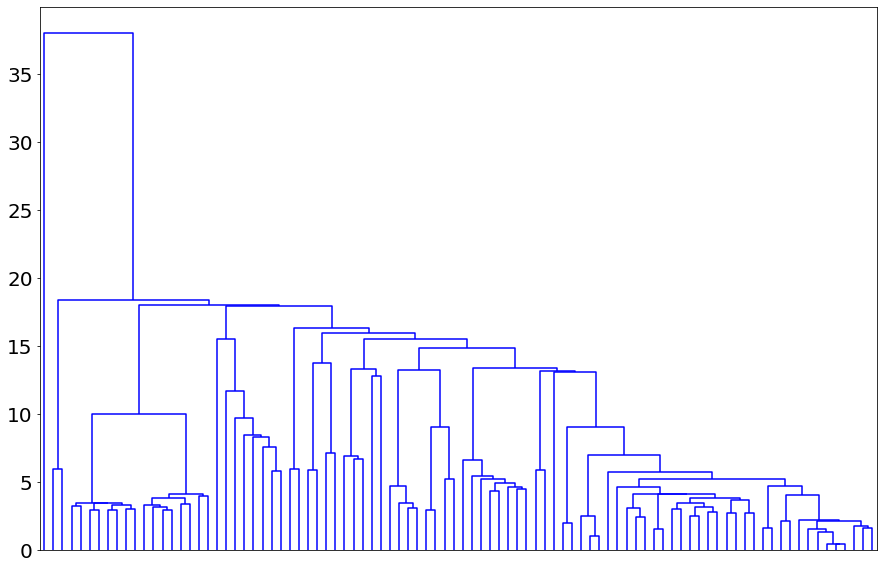
\includegraphics[width=\linewidth]{"Part 3 - Learning Systems/Unsupervised Learning/Hierarchical Clustering/figures/Agglomerative-Single.png"}
    \caption{single linkage}
  \end{subfigure}
  \begin{subfigure}[b]{0.8\linewidth}
    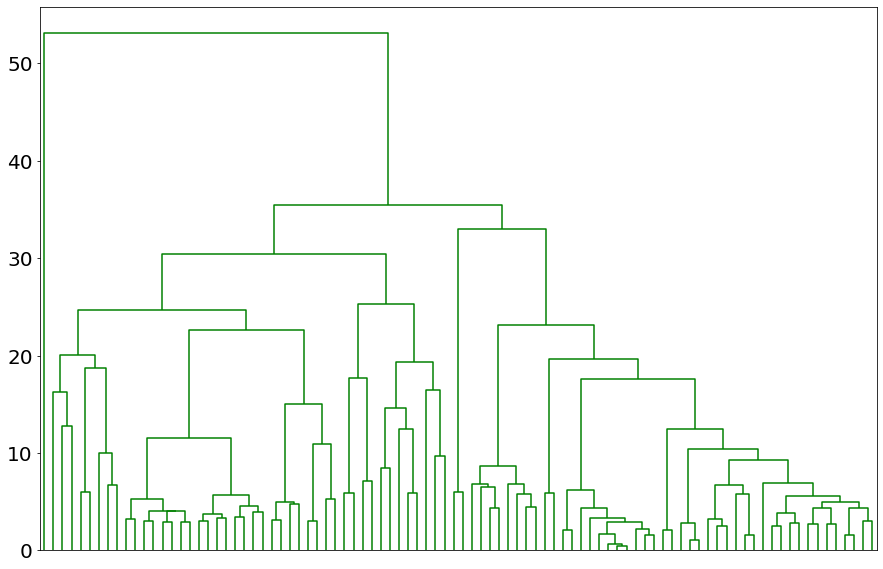
\includegraphics[width=\linewidth]{"Part 3 - Learning Systems/Unsupervised Learning/Hierarchical Clustering/figures/Agglomerative-Complete.png"}
    \caption{complete linkage}
  \end{subfigure}
  \begin{subfigure}[b]{0.8\linewidth}
    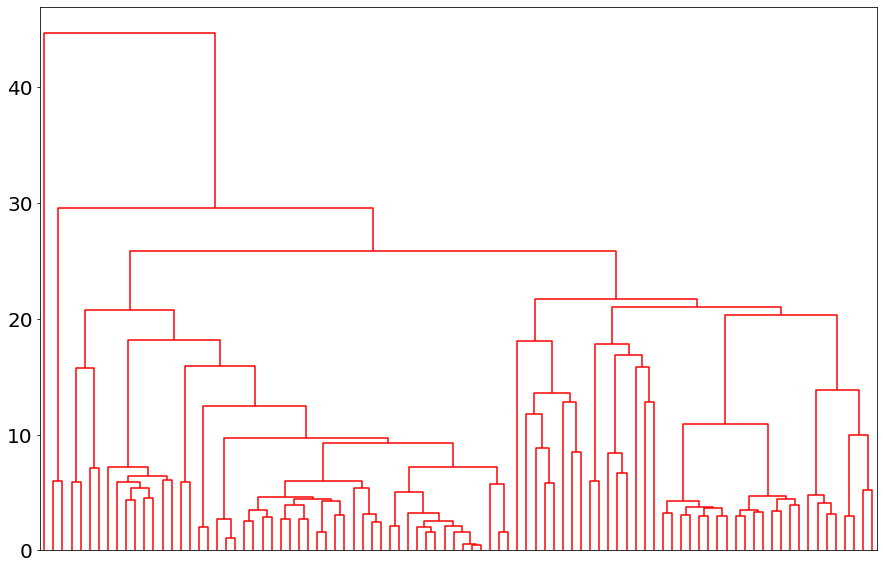
\includegraphics[width=\linewidth]{"Part 3 - Learning Systems/Unsupervised Learning/Hierarchical Clustering/figures/Agglomerative-average.png"}
    \caption{group average}
  \end{subfigure}
  \caption{Agglomerative clustering of yeast gene expressions data with (a) single linkage, (b) complete linkage and (c) group average. Figures are generated by Python. }
  \label{fig:example}
\end{figure}

\section{Summary and Discussion}

The core concepts of hierarchical clustering have been introduced. There are two types of hierarchical clustering -- agglomerative and divisive, differing in the direction of forming clusters. Agglomerative clustering starts at the bottom treating each single example in the dataset as a cluster, and recursively merges the closest pair of clusters into a single cluster. Divisive clustering starts at the top with one big cluster and recursively splits into two new groups with the largest between-group dissimilarity. Agglomerative clustering is more widely used due to its easier implementation. Same as the other clustering algorithms, hierarchical clustering requires a distance measure to decide how far an example is from another. In addition, agglomerative clustering needs to choose a dissimilarity measure to decide the distance between two clusters. Three commonly used dissimilarity measures have been discussed and compared through a yeast gene data example, which are single linkage, complete linkage and group average. The resulting clusters from hierarchical clustering are represented by a dendrogram. It is highly interpretable by showing how examples are grouped at each hierarchy level and the height of two clusters when being merged. This is also the main reason for the popularity of hierarchical clustering in the field of bioinformatics. With good explainability, it will be interesting to see how hierarchical clustering contributes to many other fields, for the readers to explore. Some inspirations may be found here~\cite{Whittaker2019}. If you are familiar with Python and would like to implement different versions of hierarchical clustering and use them on some datasets, here are some useful resources~\cite{Sklearn2022}~\cite{Brownlee2020}. 

\section*{Exercise}

\begin{enumerate}
\item Is agglomerative hierarchical clustering a deterministic or non-deterministic clustering algorithm? A deterministic algorithm always gives the same results regardless of the starting states of the algorithm. \\

\item You are using agglomerative clustering to cluster an 1-dimensional data set. At some point, you obtain 2 clusters: cluster 1 with numbers [7, 11] and cluster 2 with numbers [12, 16, 20]. What is the distance between these 2 clusters using single linkage? And what about using complete linkage and group average? \\

\item Use single and complete link agglomerative clustering to group the data described by the following distance matrix. Draw the dendrograms.

\begin{center}
\begin{tabular}{| c | c | c | c | c |}
\hline 
 & A & B & C & D \\ \hline
A & 0 & 5 & 2 & 3 \\  \hline
B & & 0 & 1 & 6 \\ \hline
C & & & 0 & 4 \\ \hline
D & & & & 0   \\ \hline
\end{tabular}
\end{center}

\item As hierarchical clustering does not explicitly tell you the number of clusters of data in results, how would you decide the most appropriate number of clusters?

\end{enumerate}

\section*{Exercise Answers}

\begin{enumerate}
\item Agglomerative clustering is a deterministic algorithm, as the result does not change with the starting states of the algorithm.  \\

\item The distance will be 1 when using the single linkage, because 11 from cluster 1 and 12 from cluster 2 are the nearest examples from the 2 clusters, and the distance between these 2 examples will be the distance of these 2 clusters. Similarly, when using complete linkage, the distance between the 2 clusters will be 13, which is the distance between examples 7 and 20. When using group average, we calculate the average distance between all pairs of examples from the two clusters, so the cluster distance will be 7. \\

\item When using the single linkage, the dendrogram is:
\begin{figure}[htp]
\centering
\captionsetup{justification=centering}
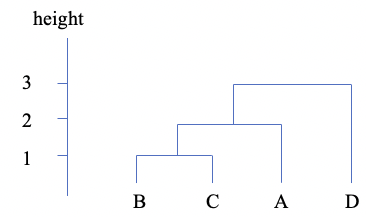
\includegraphics[width=6cm]{"Part 3 - Learning Systems/Unsupervised Learning/Hierarchical Clustering/figures/AnswerQ3-single.png"}
\caption{Resulting dendrogram from the single linkage}
\label{fig:Q3-single}
\end{figure}

When using the complete linkage, the dendrogram is:
\begin{figure}[htp]
\centering
\captionsetup{justification=centering}
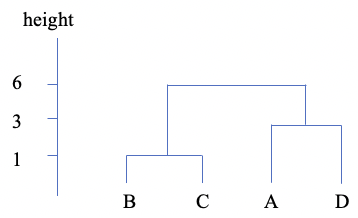
\includegraphics[width=6cm]{"Part 3 - Learning Systems/Unsupervised Learning/Hierarchical Clustering/figures/AnswerQ3-complete.png"}
\caption{Resulting dendrogram from the complete linkage}
\label{fig:Q3-complete}
\end{figure}

\item The best choice is always the pre-knowledge, if you know the number of clusters in advance. If not, a common way specific to hierarchical clustering is to observe the dendrogram you obtain. See and compare the height of every two merging clusters at each hierarchy level. Find two adjacent heights that give the largest distance increase, and draw a horizontal line between these two hierarchy levels. The best choice can be the number of vertical lines intersect by the horizontal line. Other general methods include Silhouette coefficient~\cite{Wiki2022a}, Elbow method~\cite{Baruah2020}, Calinski-Harabasz Index~\cite{Baruah2020}, Davies-Bouldin Index~\cite{Wiki2022b}, etc.
\end{enumerate}

\bibliographystyle{unsrt}
\bibliography{bibliography}
